% Motivation paragraph
\Cref{sec:hh_motivation}

In the current experimental environment of HEP, direct searches for
non-resonant Higgs boson pair production are the most sensitive probes
of the Higgs boson self-coupling constant, \lambdahhh, due to the
large sensitivity of the total and differential non-resonant \HH
production cross section to anomalous values of \lambdahhh. Hereafter,
the self-coupling constant is given in terms of the modifier
$\klambda = \lambdahhh / \lambdahhh^{\text{SM}}$ relating an assumed
value of the self-coupling constant to the value predicted by the SM.

The inclusive \HH cross section via the \ggF and VBF production modes
is shown in \Cref{fig:hh_xsec_incl} as a function of
\klambda. Non-resonant production of \HH via \ggF constitutes the
dominant contribution throughout the considered \klambda range,
exceeding the production cross section via VBF by at least a factor of
about five (18 for SM \HH production). For the \ggF production mode,
the destructive interference between the box and triangle diagram
becomes maximal for $\klambda \approx 2.3$ at which point the cross
section is at a minimum of about \SI{13}{\femto\barn}. Similar
behaviour is expected for the VBF production mode although involving
different diagrams (cf.\ \Cref{fig:hh_feynmans}) and yielding the
cross section minimum just below $\klambda = 2$.

Anomalous values of the Higgs boson self-coupling constant also change
the differential \HH production cross section, primarily affecting the
distribution of the Higgs boson pair invariant mass, \mHH. The effect
of anomalous \klambda on the shape XXXXX is shown
in~\Cref{fig:hh_xsec_mhh} for the \ggF production mode.

\begin{figure}[htbp]
  \begin{subfigure}[t]{0.485\textwidth}
    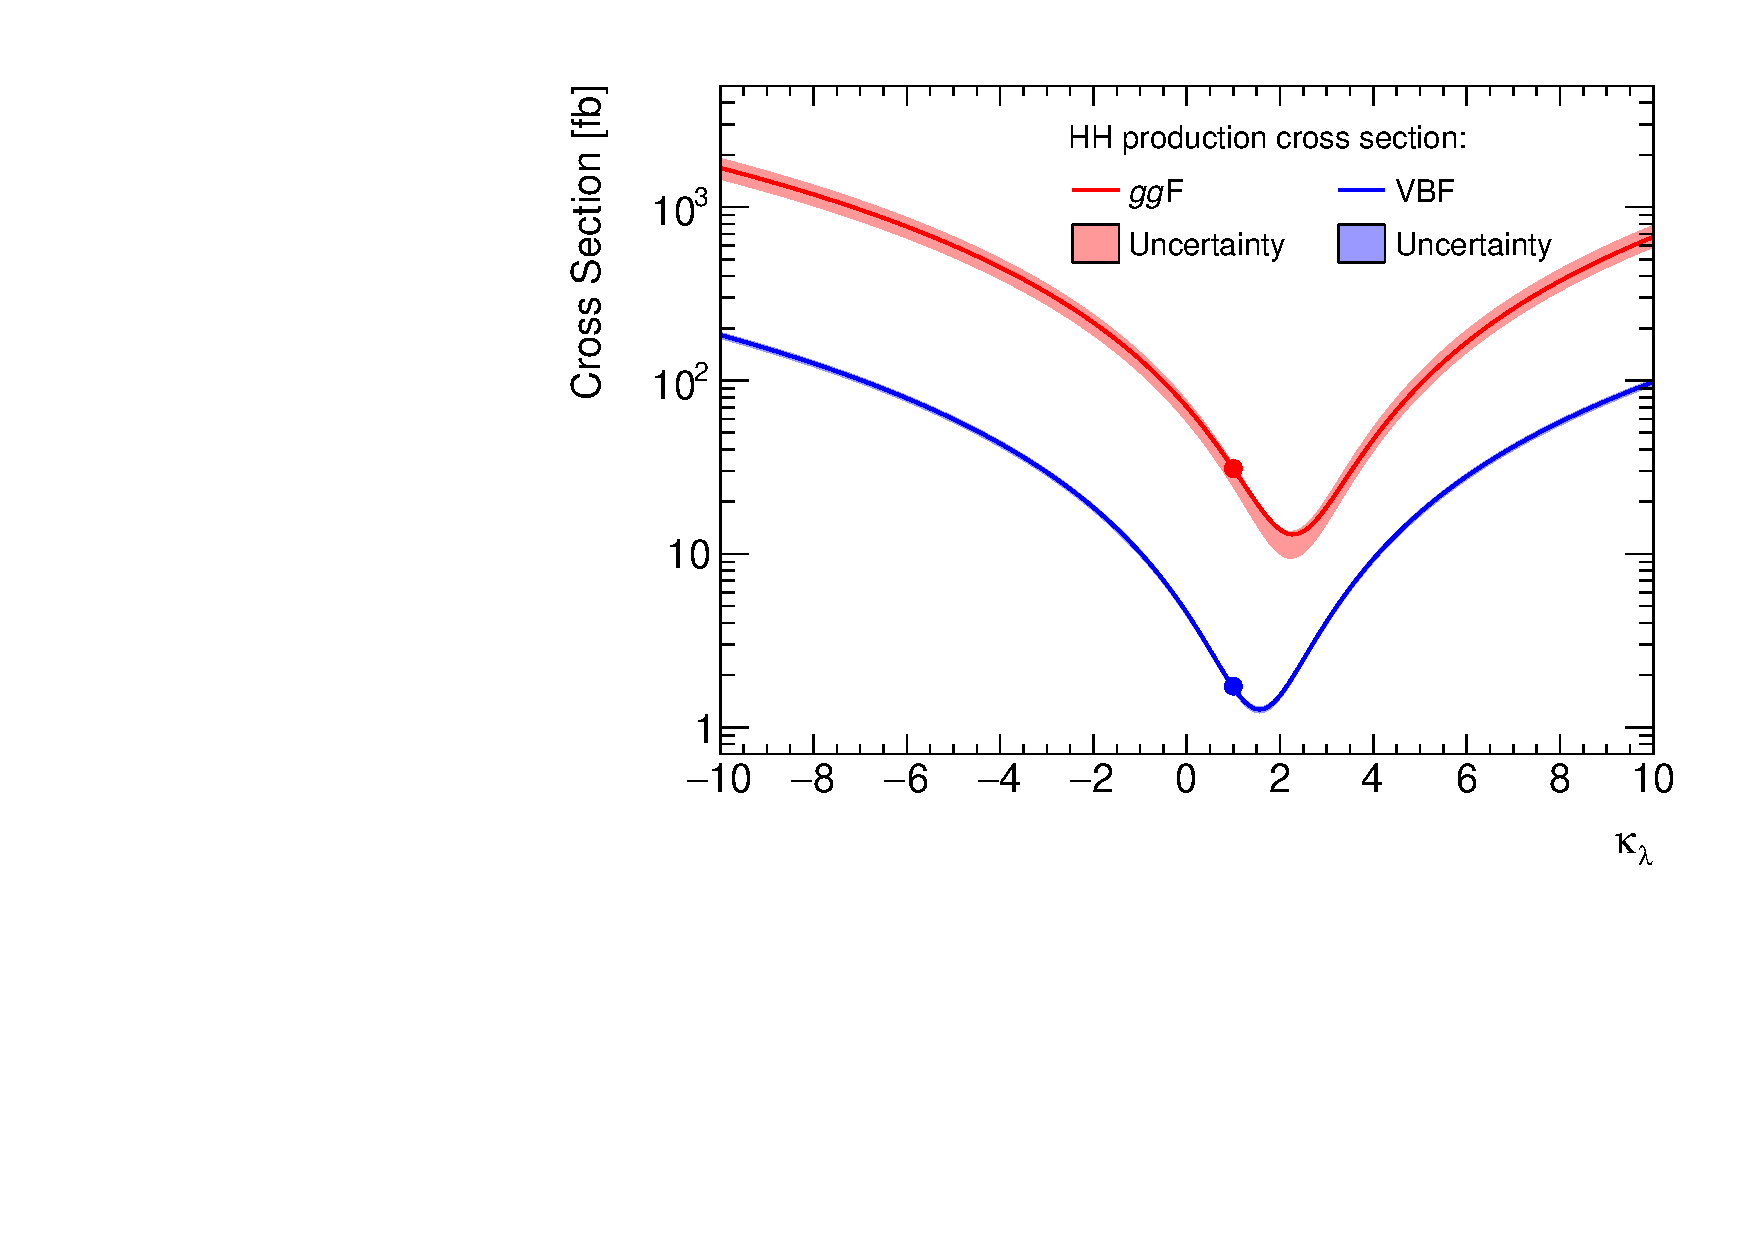
\includegraphics[width=\textwidth]{self_coupling/hh_xsec}
    \subcaption{Total \HH production cross section via \ggF and VBF as
      a function of \klambda. The production cross section via \ggF is
      given at $\text{NNLO}_{\text{NLO-i}}$ rescaled to
      $\text{NNLO}_{\text{FTapprox}}$ in the $\klambda = 1$
      limit~\cite{Amoroso:2020lgh,Baglio:2020wgt,LHCHWGHH,Grazzini:2018bsd}. The
      production cross section via VBF is obtained from simulation
      with \MGNLO at LO after applying an $\text{N}^3\text{LO}$
      $k$-factor derived for the SM
      case~\cite{Dreyer:2018qbw,LHCHWGHH}. The cross sections are
      parameterised as quadratic functions of \klambda. Theoretical
      uncertainties are shown as coloured bands.}%
    \label{fig:hh_xsec_incl}
  \end{subfigure}\hfill%
  \begin{subfigure}[t]{0.485\textwidth}
    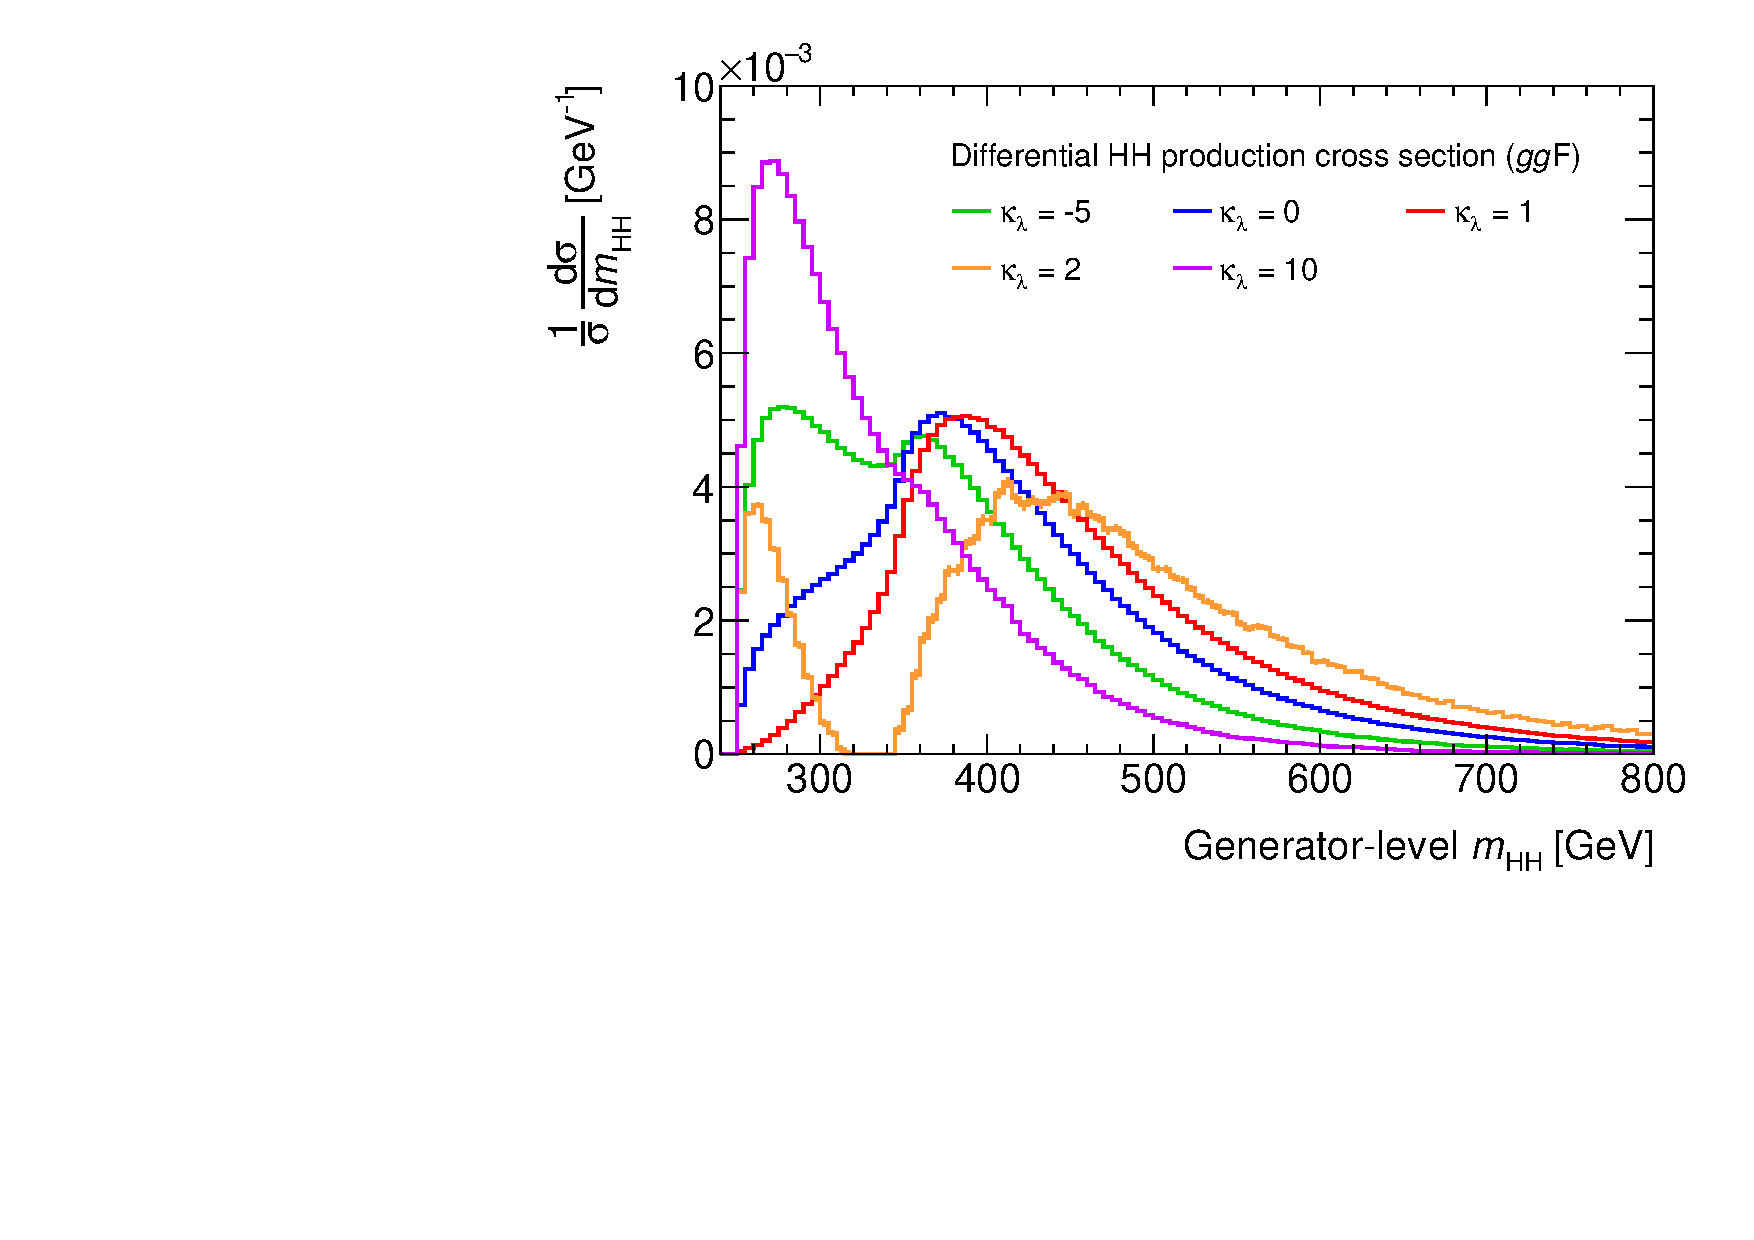
\includegraphics[width=\textwidth]{self_coupling/hh_mhh_vs_klam}
    \subcaption{Differential \HH production cross section with respect
      to \mHH at generator-level for the \ggF production mode and
      selected values of \klambda. The cross sections are obtained
      from simulation with \POWHEGBOX[v2] at NLO including the
      top-quark mass
      dependence~\cite{Heinrich:2019bkc,Heinrich:2020ckp} for
      $\klambda = 0, 1, 10$. For $\klambda = -5, 2$, the differential
      cross sections are estimated using morphing techniques derived
      at LO~\cite{ATL-PHYS-PUB-2019-007}. The differential cross
      sections are normalised by dividing by the total cross
      section. Only statistical uncertainties from the finite number
      of generated events are shown.}%
    \label{fig:hh_xsec_mhh}
  \end{subfigure}

  \caption{Variation of the total (a) and differential (b) Higgs boson
    pair production cross section with \klambda for
    $\mH = \SI{125.0}{\GeV}$ in $pp$-collisions at
    $\sqrt{s} = \SI{13}{\TeV}$. A description of the total cross
    section and morphing techniques used to obtain differential
    predictions for arbitrary \klambda is given in~\Cref{TODO}.}%
  \label{fig:hh_xsec_vs_klam}
\end{figure}

The results from the search for non-resonant Higgs bosons pair
production presented in~\Cref{sec:dihiggs} was reinterpreted by the
ATLAS collaboration in the context of possible variations of the Higgs
boson self-coupling constant \lambdahhh in
Ref.~\cite{ATLAS-CONF-2021-052}.


The total Higgs boson pair production cross section with anomalous
couplings. Following recommendations by the LHC Higgs Working
Group~\cite{LHCHWGHH}:
\begin{description}

\item[\ggF production mode] The cross sections of \HH production with
  anomalous self-couplings were calculated in
  Ref.~\cite{Amoroso:2020lgh} at $\text{NNLO}_{\text{NLO-i}}$
  (NLO-improved). This prediction is obtained from combining the
  result with the full top-quark mass dependence at
  NLO~\cite{Buchalla:2018yce}


  with NNLO corrections in the $m_{t} \to \infty$
  limit~\cite{deFlorian:2017qfk}.

  Additionally, the prediction is rescaled such that it coincides with
  the SM \HH cross section at $\text{NNLO}_{\text{FTapprox}}$ at
  $\klambda = 1$.

  The total \HH production cross section via \ggF was found to depend
  quadratically on \klambda and is thus parameterised
  accordingly~\cite{LHCHWGHH}.

\item[VBF production mode]

\end{description}

\todo[inline]{Should say that this re-interpretation was generally
  considered while developing the analysis outlined in the previous
  chapter.}

anomalous couplings

Self-coupling modifier~$\klambda = \lambdahhh / \lambdahhh^{\text{SM}}$.

\todo[inline]{Read YR about Higgs cross section predictions:
  \url{https://cds.cern.ch/record/2227475/files/CERN-2017-002-M.pdf}}

Sample combination method:~\cite{ATL-PHYS-PUB-2019-007}



\todo[inline]{Hadhad channel: Acceptance times efficiency vs mHH.}

\todo[inline]{Hadhad channel: Acceptance times efficiency vs kLambda.}


\begin{figure}[htbp]
  \centering

  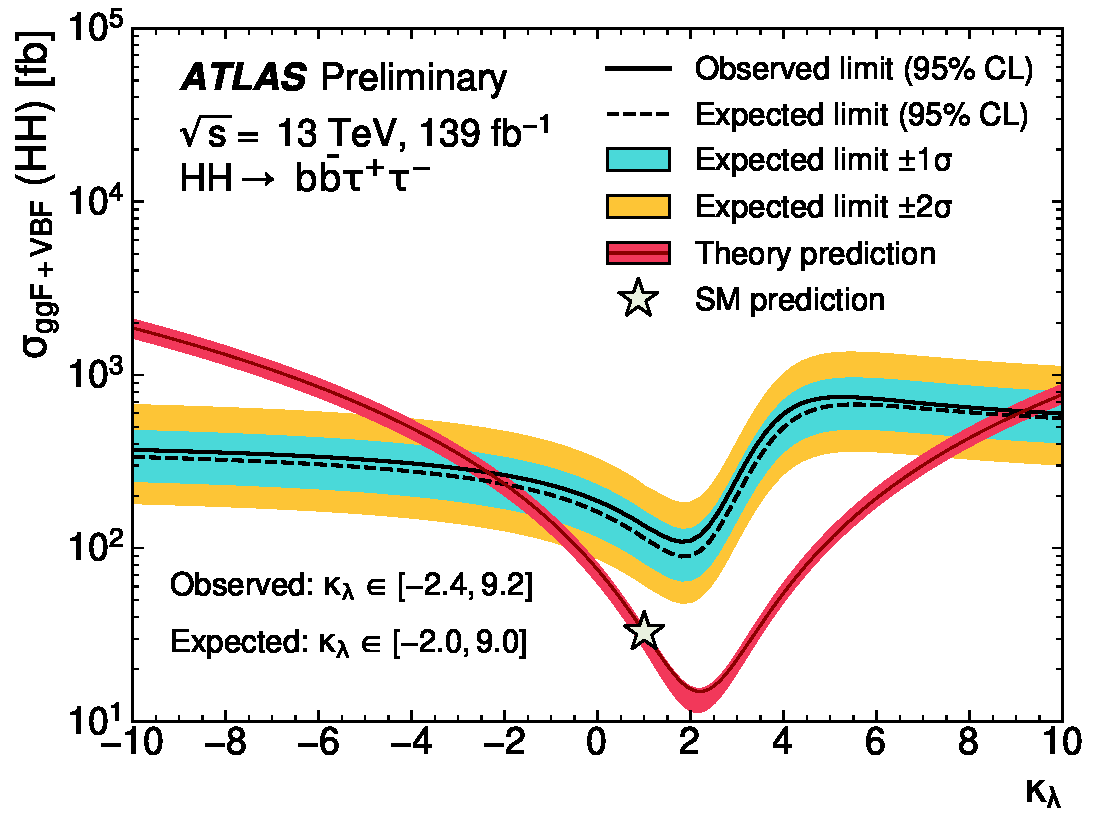
\includegraphics[width=0.6\textwidth]{self_coupling/klam_scan_result}

  \caption{Klambda scan. The figure is taken from
    Ref.~\cite{ATLAS-CONF-2021-052}.}%
  \label{fig:klambda_scan}
\end{figure}


\todo{Updated result from H+HH
  combination~\cite{ATLAS-CONF-2022-050}.}


%%% Local Variables:
%%% mode: latex
%%% TeX-master: "../../phd_thesis"
%%% End:
